\documentclass[a4paper,french]{paper}
\usepackage{../../../../../_assets/latex/5N_OPTO_ELEC}

%Informations about this document 
%------------------------------------------
\def\module{Opto-Electronique - S5}
\def\moduleAbrege{5N-027-SCI / OptoElec}
\def\annee{}

\def\titre{Séance 1 / Bases et amplificateur linéaire}
\author{Julien VILLEMEJANE}

\subtitle{Séance 1}
\institution{LEnsE / Institut d'Optique Graduate School}

\title{\titre}
\begin{document} 
%Beginning First Page. 
%------------------------------------------
\enteteThematiqueObligatoire{}

\textit{Pour ce TD, on pourra s'appuyer sur les fiches résumées} :  \href{https://lense.institutoptique.fr/ressources/Annee1/Electronique/fiches/2020_FR_Fondamentaux.pdf}{Fondamentaux} et \href{https://lense.institutoptique.fr/ressources/Annee1/Electronique/fiches/2021_FR_ALI.pdf}{Ampli Linéaire Intégré}.

%Beginning Content. 
%------------------------------------------

%%%%%%%%%%%%%%%%%%%
%%%%%%%%%%%%%%%%%%%
\encadreTDExo{1.1 - Abaisser une tension}{
Proposez un circuit permettant d'abaisser une tension d'un facteur $k$.

$0 < k < 1$ 
}
%%%%%%%%%%%%%%%%%%%
Pour réduire une tension, il est possible d'utiliser un \textbf{pont diviseur de tension}, basé sur l'utilisation de 2 résistances en série comme proposé dans le schéma suivant.

\medskip

\begin{center}
\begin{circuitikz}
	\draw (1,0) to [short, *-] (3,0)
		to[R=$R_{2}$, -*] (3,2)
		to[R=$R_{1}$, -] (3,4)
		to [short, -*, i<_=$I$] (0,4);
	\draw (3,0) to[short, -o] (4,0);
	\draw (3,2) to[short, -o, i=$I_S$] (4,2);
	
	% fleche
	\draw (0,0.5) edge[->] (0,3.5);
	\node (Ein) at (-1,2.25){$V_E$};

	\draw (0,0) to [short, *-] (1,0)
		node[ground](GND){};
	% fleche
	\draw (3.5,0.3) edge[->, green!40!black] (3.5,1.7); \node[text=green!40!black] (US) at (4,1){$V_S$};
\end{circuitikz}
\end{center}

Pour le calcul, on peut s'intéresser au courant $I$ en écrivant deux lois des mailles différentes :

\begin{enumerate}
	\item $V_E - R_1 \cdot I - R_2 \cdot I = 0$
	\item $V_S - R_2 \cdot I = 0$
\end{enumerate}

Cela suppose que l'on considère que le courant $I_S = 0$.

En combinant les deux, on obtient la relation entre $V_E$ et $V_S$ suivante : $$\boxed{V_S = V_E \cdot \frac{R_2}{R_1 + R_2}}$$

\noindent\hrulefill

\newpage

Si on suppose maintenant que le circuit précédent est chargé par une résistance $R_L$, on obtient alors le montage suivant :

\begin{center}
\begin{circuitikz}
	\draw (1,0) to [short, *-] (3,0)
		to[R=$R_{2}$, -*, i<_=$I_2$] (3,2)
		to[R=$R_{1}$, -] (3,4)
		to [short, -o, i<_=$I$] (0,4);
	\draw (3,0) to[short, -o] (4,0);
	\draw[dashed] (4,0) to[short, -] (5.5,0) 
		to[R=$R_L$, -] (5.5,2)
		to[short, -] (4,2);
	\draw (3,2) to[short, -o, i=$I_S$] (4,2);
	
	% fleche
	\draw (0,0.5) edge[->] (0,3.5);
	\node (Ein) at (-1,2.25){$V_E$};

	\draw (0,0) to [short, o-] (1,0)
		node[ground](GND){};
	% fleche
	\draw (3.5,0.3) edge[->, green!40!black] (3.5,1.7); \node[text=green!40!black] (US) at (4,1){$V_S$};
\end{circuitikz}
\end{center}

Dans ce cas, le courant $I_S$ n'est plus nul.

Le courant $I$ traversant $R_1$ va alors se partager entre $R_2$ et $R_L$. On aura alors la seconde loi des mailles écrites précédemment qui ne sera plus valide.

On peut alors écrire les relations suivantes :
\begin{enumerate}
	\item loi des mailles : $V_E - R_1 \cdot I + V_S$ 
	\item loi des mailles : $V_S - R_L \cdot I_S = 0$  
	\item loi des noeuds : $I = I_S + I_2$ 
	\item loi des mailles : $V_S - R_2 \cdot I_2 = 0$
\end{enumerate}

Après regroupement et simplification, on obtient la relation suivante : $$\boxed{V_S = V_E \cdot \frac{R_{eq}}{R_1 + R_{eq}}}$$  

avec $R_{eq} = \frac{R_2 \cdot R_L}{R_2 + R_L}$ (mise en parallèle de $R_2$ et $R_L$).
 
%%%%%%%%%%%%%%%%%%%
%%%%%%%%%%%%%%%%%%%
\encadreTDExo{1.2 - Courants et tensions}{

Soit le circuit suivant :

\begin{center}
\begin{circuitikz}
\draw (0,0) to[I, l=$I_{PHD}$, invert] (0,3)
	to[short, -*, i=$I_{PHD}$] (2,3)
	to[R, R=$Z_{PHD}$, -*] (2,0)
	to[short] (0,0);
	
\draw (1,0) to[short, *-] (1,0) node[ground] {};
\draw (2,3) to[short, -*] (4,3) to[R, R=$R_{PHD}$, -*] (4, 0)
	-- (2,0);

\draw (4,3) to[short, -*] (6,3) to[R, R=$R_{e}$, -*] (6, 0)
	-- (4,0);

\draw (6,3) -- (8,3) to[R, R=$Z_{e}$] (8,0) -- (6,0);
\end{circuitikz}
\end{center}

\begin{enumerate}
	\item Donnez l'expression de $V_S$ en fonction de $I_{PHD}$.
	\item Que devient cette expression si $R_e \longrightarrow +\infty$, $Z_e \longrightarrow +\infty$ et $Z_{PHD} \longrightarrow +\infty$ ?
	
	\medskip 
	
	On se place à présent en régime harmonique.
	
	$Z_{PHD} $ est une capacité $C_{PHD} $ et $Z_e$ est une capacité $C_e$.
	
	\item Que devient l'expression de $V_S$ en fonction de $I_{PHD}$ ?
	\item A quoi peuvent correspondre l'ensemble des éléments du montage ?
	
\end{enumerate}

}
%%%%%%%%%%%%%%%%%%%
\textbf{Question 1}
	
Les 5 branches sont en parallèle et sont soumises à la même différence de potentiel $V_S$.

Le courant $I_{PHD}$ se distribue dans les 4 autres branches : $I_{PHD} = \frac{V_S}{Z_{PHD}} + \frac{V_S}{R_{PHD}} + \frac{V_S}{Z_{e}} + \frac{V_S}{R_{e}}$

Ainsi : $$V_S = \frac{I_{PHD}}{\frac{1}{Z_{PHD}} + \frac{1}{R_{PHD}} + \frac{1}{Z_{e}} + \frac{1}{R_{e}}}$$


\textbf{Question 2}

L'expression précédente devient : $V_S = R_{PHD} \cdot I_{PHD}$

\textbf{Question 3}

$Z_{PHD} = \frac{1}{j \cdot C_{PHD} \cdot \omega}$ et $Z_{e} = \frac{1}{j \cdot C_{e} \cdot \omega}$ 

L'expression de la question 1 devient alors : $$\frac{V_S}{I_{PHD}} = \frac{1}{\frac{1}{R_{PHD}} + j \cdot C_{PHD} \cdot \omega + \frac{1}{R_{e}} + j \cdot C_{e} \cdot \omega}$$

On pose : $R_k = \frac{R_e \cdot R_{PHD}}{R_e + R_{PHD}}$ et $C_k = C_{PHD} + C_e$

Après simplification : $$\frac{V_S}{I_{PHD}} = R_k \cdot \frac{1}{1 + j \cdot R_k \cdot C_k \cdot \omega}$$

\textbf{Question 4}
	
Une \textbf{photodiode} peut être modélisée par une source de courant, dépendant du flux lumineux qu'elle reçoit, et d'une capacité parasite $C_{PHD}$.

De l'autre côté, il est possible de modéliser un oscilloscope, permettant de visualiser le signal électrique, par une résistance d'entrée $R_e$ et le cable coaxial, qui permet d'amener le signal jusqu'à l'entrée de l'oscilloscope, par un condensateur de capacité $C_e$.

Enfin, la résistance $R_{PHD}$ permet de transformer le courant résultant de la photodiode en une tension plus facilement visualisable à  l'aide d'un oscilloscope.

%%%%%%%%%%%%%%%%%%%
%%%%%%%%%%%%%%%%%%%
\encadreTDExo{1.3 - Amplificateur linéaire intégré}{
On fournit en annexe une partie de la documentation technique de l'amplificateur linéaire intégré (ALI) \textbf{TL081}.

\begin{enumerate}
	\item Cherchez dans la documentation les valeurs des paramètres électriques suivants :
	\begin{enumerate}
		\item Tension d'alimentation (Supply Voltage)
		\item Tension d'entrée différentielle maximale
		\item Amplification différentielle 
		\item Gain unitaire ou produit gain-bande-passante
		\item Impédance d'entrée 
		\item Slew Rate
	\end{enumerate}
	\item Précisez à quoi corresponde chacun de ces paramètres.
	\item Rappelez la relation entre les entrées $V^+$, $V^-$ et la sortie $V_S$ d'un ALI.
	\item Tracez la caractéristique $V_S = f (\varepsilon)$ où $\varepsilon = (V^+ - V^-)$ pour cet ALI avec $V_{CC} = 15\operatorname{V}$.
	\item Est-ce un bon amplificateur ? Quelle est sa bande-passante ?

\end{enumerate}
}


%%%%%%%%%%%%%%%%%%%
\textbf{Question 1}

\begin{itemize}
	\item Tension d'alimentation (Supply Voltage) = 18V
	\item Tension d'entrée différentielle maximale = 30V
	\item Amplification différentielle - $A_{VD} = 200\operatorname{V/mV} = 2 \cdot 10^5$
	\item Gain unitaire ou produit gain-bande-passante - $B_1 = 3\operatorname{MHz}$ 
	\item Impédance d'entrée - $r_i = 10^{12}\operatorname{\Omega} = 10^6\operatorname{M\Omega} = 1\operatorname{T\Omega}$
	\item Slew Rate - $SR = 13\operatorname{V/\mu{}s}$
\end{itemize}

\textbf{Question 2}

\begin{itemize}
	\item Tension d'alimentation : les ALI sont des composants actifs, ils nécessitent une source d'énergie pour fonctionner. Ici il est nécessaire de réaliser une source de tension symétrique, c'est à dire une source positive $+V_{CC}$ et une source négative $-V_{CC}$, où $V_{CC} < 18\operatorname{V}$
	\item Tension d'entrée différentielle maximale : c'est la différence de potentiel maximale admissible entre $V^+$ et $V^-$. On appelle tension d'entrée différentielle $\varepsilon = (V^+ - V^-)$
	\item Amplification différentielle : c'est l'amplification du composant, le lien entre la tension de sortie ($V_S$) et la tension différentielle d'entrée ($\varepsilon$).
	\item Gain unitaire ou produit gain-bande-passante : c'est une donnée essentielle qui permet de connaître la bande-passante du composant lorsque l'amplification du montage est de 1. Sur les montages amplificateurs (à base d'ALI), le produit amplification bande-passante est constant. 
	\item Impédance d'entrée : c'est l'impédance vu par le montage en amont de l'ALI.
	\item Slew Rate : cette donnée caractérise la pente maximale que pourra avoir l'ALI en sortie.
\end{itemize}

\textbf{Question 3}

$$V_S = A_{VD} \cdot (V^+ - V^-)$$

avec $A_{VD} = 200\operatorname{V/mV} = 2 \cdot 10^5$ (dans le cas du TL081).

\textbf{Question 4}

Courbe avec saturation à +/-15V (dans le cas d'une alimentation où $V_{CC} = 15\operatorname{V}$. 

La saturation en sortie apparait pour une valeur de $\varepsilon = V_{CC} / A_{VD}$. Pour $V_{CC} = 15\operatorname{V}$, on a $\varepsilon_{MAX} = V_{CC} / A_{VD} = 75\operatorname{\mu{}V}$.

\textbf{Question 5}

L'amplication différentielle est souvent supérieure à $10^5$, c'est donc un très bon amplificateur.

Cependant, il a un produit amplification/bande-passante ($GBW$) qui est constant et "faible", ce qui le rend finalement peu efficace pour des fréquences élevées en boucle ouverte.

Par exemple, pour un $GBW = 3\operatorname{MHz}$ et une amplification différentielle $A_{VD} = 2 \cdot 10^5$ (cas du TL081), on obtient une bande-passante en boucle ouverte (sans rebouclage) $f_c = GBW / A_{VD} = 15\operatorname{Hz}$.


%%%%%%%%%%%%%%%%%%%
%%%%%%%%%%%%%%%%%%%
\encadreTDExo{1.4 - Amplificateur inverseur}{
On se propose d'étudier à présent le montage suivant :

\begin{center}
\begin{circuitikz} 
	\node [op amp, fill=blue!10!white](A1) at (0,0){\texttt{AOP1}};
	\draw (A1.-) to[short] ++(-.5,0) coordinate(A) to[short] ++(0,1.5) coordinate(B) to[R=$R_2$] (B -| A1.out) to[short, -*] (A1.out);
	\draw (A1.-) to[short,-*] ++(-.5,0) coordinate(AA) to[R=$R_1$] ++(-2.5,0) coordinate(BB) to[short,-o] ++(-.5,0) coordinate(CC);
	\draw (A1.+) to[short] ++(0,-0.5) node[ground]{};
	\draw (A1.out) to[short,-o] ++(1,0) coordinate(D);
	\draw (-4.6,-1) edge[->,color={green!40!black}] (-4.6,0.3);
	\node[text={green!40!black}] (Ve) at (-5.1,-0.35){$V_e$}; 
	\draw (-4.6,-1.3)  to[open,-o] ++(0,0) node[ground](GND){};
	\draw (2.2,-1) edge[->, color={red}] (2.2,-0.3);
	\node[text={red}] (Vs) at (1.7,-0.6){$V_s$}; 
	\draw (2.2,-1.3)  to[open,-o] ++(0,0) node[ground](GND){};
	
\end{circuitikz}
\end{center}

\begin{enumerate}
	\item Donnez la relation entre $V_S$ et $V_E$ du circuit précédent en utilisant la relation d'entrées-sortie de l'exercice 1.
	\item Quelle hypothèse fait-on souvent lorsqu'on utilise des ALI avec une rétroaction négative ?
	\item Quelle relation trouve-t-on alors entre $V_S$ et $V_E$ en partant de cette hypothèse ?
	\item Cette hypothèse est-elle justifiée ?
\end{enumerate}

}

%%%%%%%%%%%%%%%%%%%
\textbf{Question 1}

On calcule d'abord les potentiels $V^+$ et $V^-$ en entrée de l'ALI (théorème de Millman) :

$$V^- = \frac{\frac{V_S}{R_2} + \frac{V_E}{R_1}}{\frac{1}{R_2} + \frac{1}{R_1}} = \frac{V_S \cdot R_1}{R_1 + R_2} + \frac{V_E \cdot R_2}{R_1 + R_2}$$

$$V^+ = 0$$

De plus, on sait que $V_S = A_{VD} \cdot (V^+ - V^-)$

On obtient alors : $$V_S = - A_{VD} \cdot \frac{\frac{V_S}{R_2} + \frac{V_E}{R_1}}{\frac{1}{R_2} + \frac{1}{R_1}} = \frac{V_S \cdot R_1}{R_1 + R_2} + \frac{V_E \cdot R_2}{R_1 + R_2}$$

Ce qui donne : $$T = \frac{V_S}{V_E} = - \frac{R_2}{R_1} \cdot \frac{A}{A + \frac{R_1 + R_2}{R_1}}$$


\textbf{Question 2}

$V^+ = V^-$

Lorsqu'on reboucle la sortie sur l'entrée négative sur un ALI, on change son régime de fonctionnement. Il s'agit d'un système bouclé (ou asservi). La sortie va chercher à suivre un signal de consigne appliqué sur l'entrée positive et ainsi l'erreur commise ($V^+ - V^-$) va tendre vers 0.


\textbf{Question 3}

Les relations obtenues dans la question 1 pour $V^+$ et $V^-$ restent vraies. Ainsi : 
$$V^- = \frac{\frac{V_S}{R_2} + \frac{V_E}{R_1}}{\frac{1}{R_2} + \frac{1}{R_1}} = \frac{V_S \cdot R_1}{R_1 + R_2} + \frac{V_E \cdot R_2}{R_1 + R_2}$$

$$V^+ = 0$$

De plus, en faisant l'hypothèse $V^+ = V^-$, on obtient : $$T = \frac{V_S}{V_E} = - \frac{R_2}{R_1}$$

\textbf{Question 4}

On passe de l'expression obtenue à la question 1 à celle de la question 3 lorsqu'on suppose que $A_{VD} >> \frac{R_1 + R_2}{R_1}$.

Il est fréquent de prendre des valeurs de résistances telles que $R_2 / R_1 \approx 10$. Cette hypothèse est avérée dans le majorité des cas.


\textbf{Exemple}

On souhaite montrer ici l'erreur commise sur la valeur de l'amplification entre la formule complète (incluant l'amplification différentielle) et l'approximation faite en régime linéaire, en fonction de l'amplification $R_2 / R_1$ voulue pour le système.

Pour cela, on fixe $A_{VD} = 15 \cdot 10^3$ la valeur minimale que l'on trouve dans la documentation technique du TL081 (par exemple) et on fait varier le rapport $R_2 / R_1$ de $2$ à $10^3$.

Il est possible de faire réaliser ce calcul par le script \textbf{Matlab} suivant :

\begin{lstlisting}[style=Matlab-editor]
R2 = logspace(0, 3, 101); 	R1 = 1; 	A = 15e3;
k = (R2 + R1) ./ R1;  	
m = -R2./R1

T = m * A ./ (A + k);		
erreur = (m - T) ./ m * 100;

figure;		
subplot(2,1,1);
semilogx(R2./R1, -R2./R1, R2./R1, T);
legend('Amplification avec A','Amplification simplifiee');
title('Amplificateur inverseur');		
ylabel('Amplification');

subplot(2,1,2);
semilogx(R2./R1, erreur);
ylabel('Erreur relative (\%)');		
xlabel('R2/R1');
\end{lstlisting}

On obtient alors la figure suivante : 

\begin{center}
	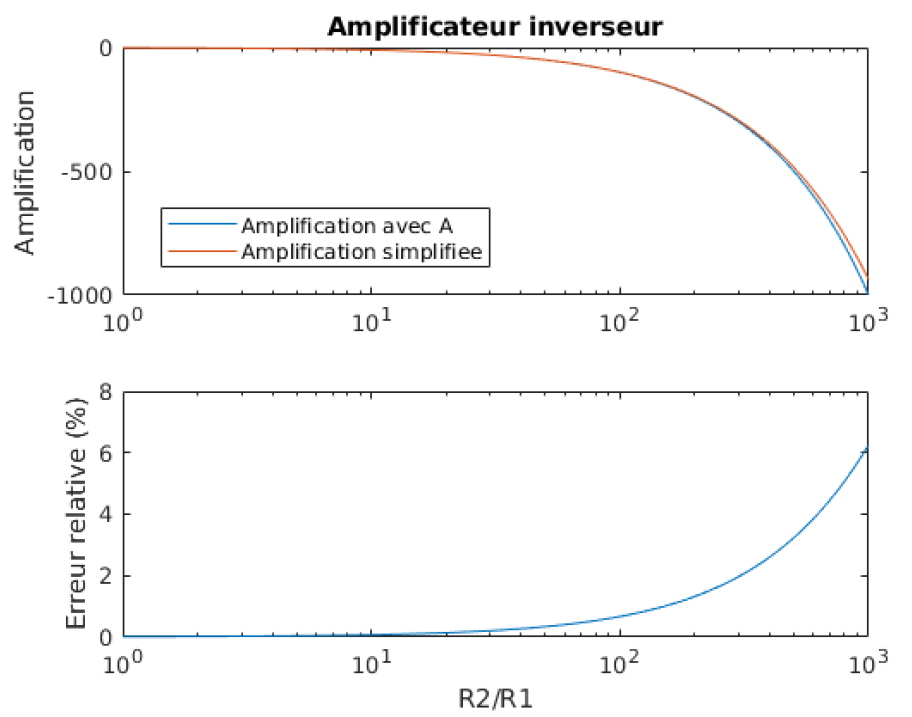
\includegraphics[width=8cm]{images/ampliinv_002_cor_a.png}
\end{center}


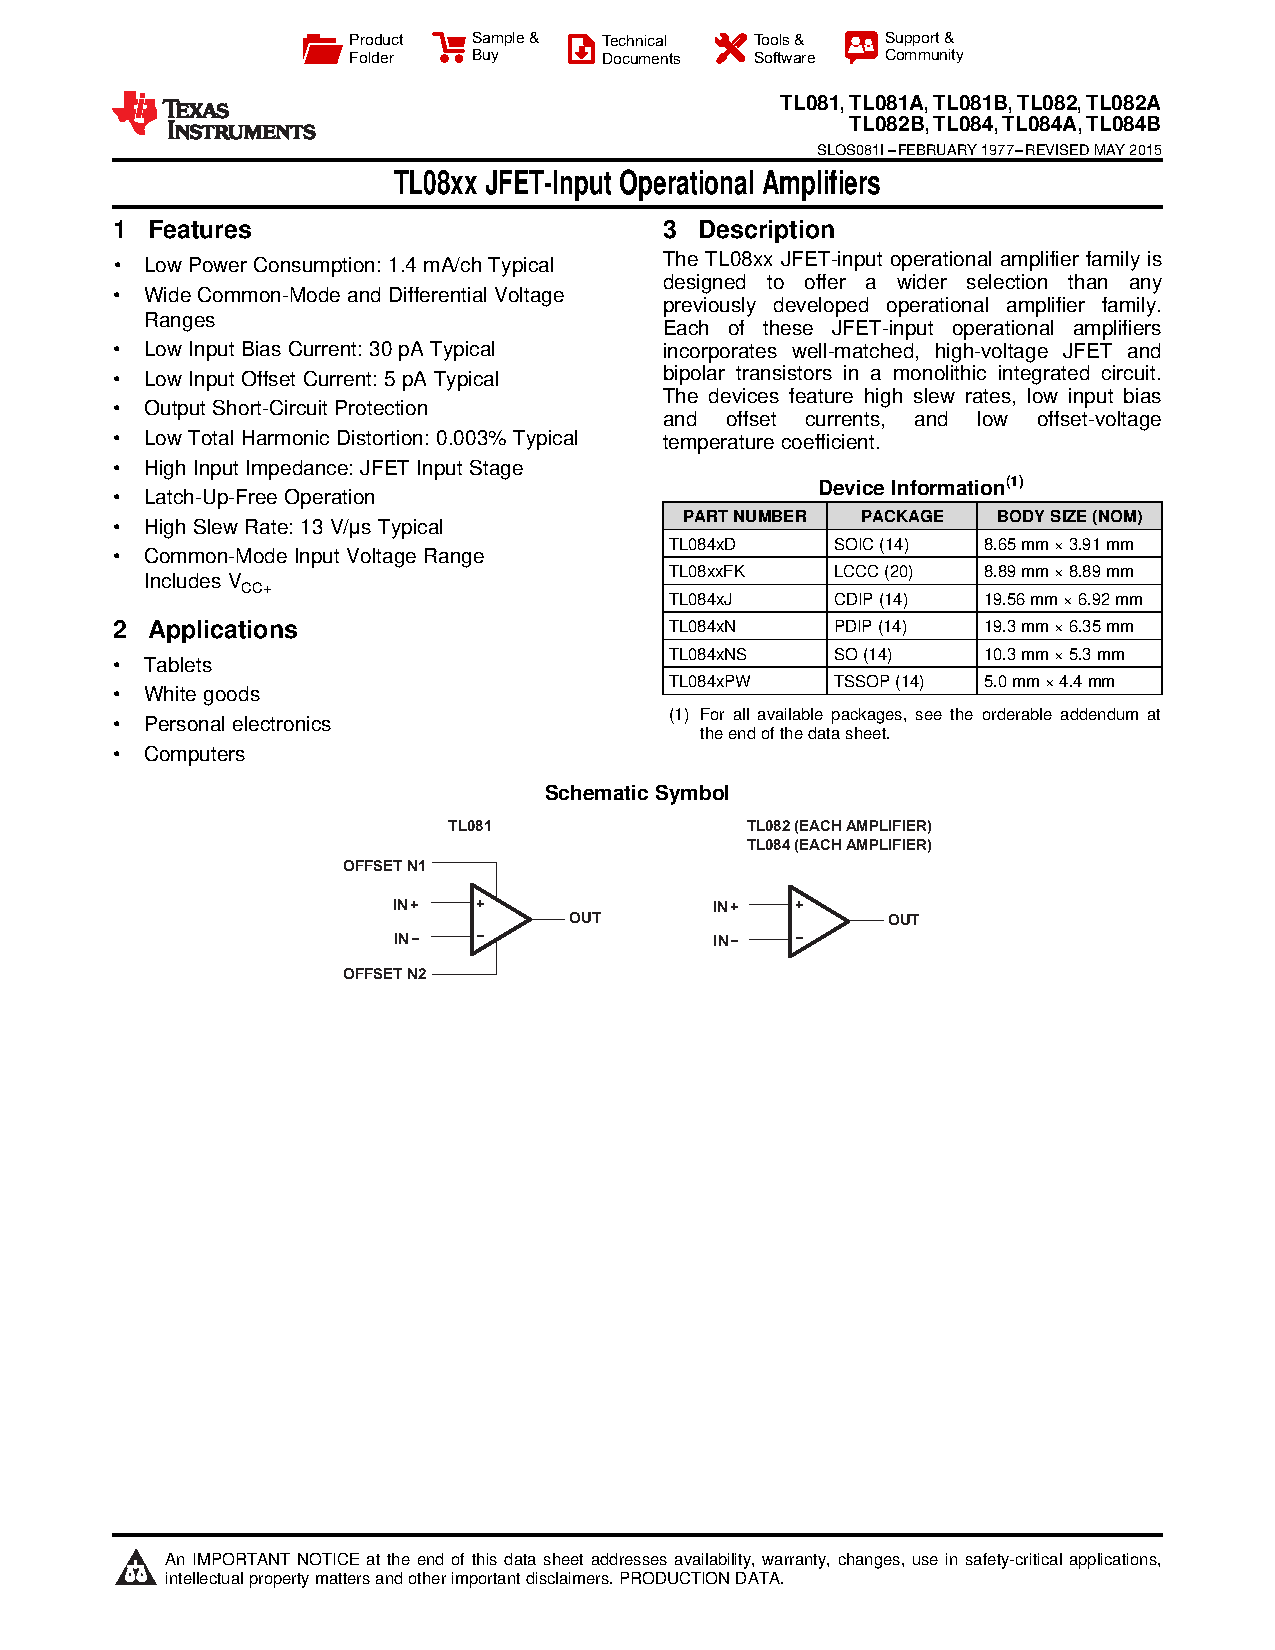
\includepdf[pages=-]{docs/doc_TL071_1p.pdf}

\end {document}